\chapter{Classification based on malware's meta-data using decision tree approach}\label{chap:4}
%EXPERIMENTAL RESULTS AND ANALYSIS
%
%
This chapter describes Win32 executive files structure, known as PE files structure, that used in classification system as malware meta-data. Afterwards, the machine learning technique, known as decision tree method, that used in classification malware system is described. Finally, this chapter presents classification based on malware's meta-data using decision tree approach. 

\section{PE file format}
\subsection{PE file overview}
\begin{figure}[h!]
\centering
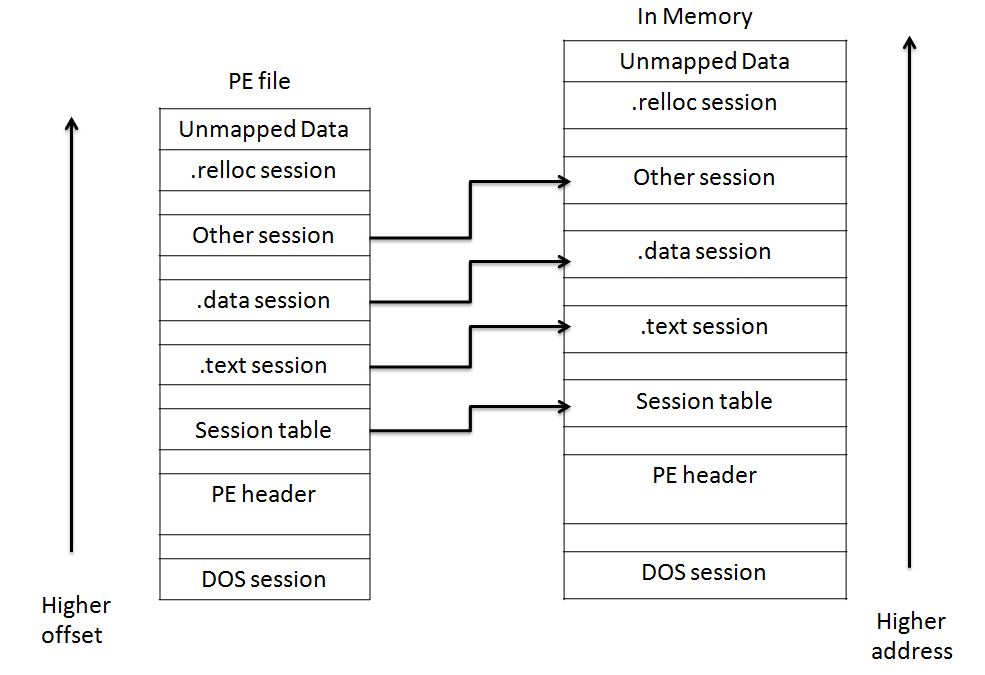
\includegraphics[width=1\textwidth]{graph/pe1.png}
\caption{PE file format.}
\label{fig:pe1}
\end{figure}

The real content of the PE file is divided into blocks called sections. A section is nothing more than a block of data with common attributes such as code/data, read/write etc. You can think of a PE file as a logical disk. The PE header is the boot sector and the sections are files in the dvisk. The files can have different attributes such as read-only, system, hidden, archive and so on. When the PE loader maps the sections into memory, it examines the attributes of the sections and gives the memory block occupied by the sections the indicated attributes.

If the PE file format is viewed as a logical disk, the PE header as the boot sector and the sections as files. Each structure contains the information about each section in the PE file such as its attribute, the file offset, virtual offset. If there are 5 sections in the PE file, there will be exactly 5 members in this structure array. Each member of the array is equivalent to the each directory entry in the root directory.

That's all about the physical layout of the PE file format. The major steps in loading a PE file into memory is described as follow:

\begin{itemize}
\item When the PE file is running, the PE loader examines the DOS MZ header for the offset of the PE header. If it is found, it would skip to the PE header.
\item The PE loader checks if the PE header is valid. If so, it goes to the end of the PE header.
\item Following the PE header is the section table. The PE header reads information about the sections and maps those sections into memory using file mapping. It also gives each section the attributes as specified in the section table.
\item After the PE file is mapped into memory, the PE loader concerns itself with the logical parts of the PE file, such as the import table.
\end{itemize}

The above steps are oversimplification and are based on my own observation. There may be some inaccuracies but it should give you the clear picture of the process.
\subsection{PE header}

PE header of second part of PE files structure. PE header includes important information of ma . As shown in Figure \ref{fig:peheader} PE header consists of four parts, a MS-DOS section, PE header, a section table, images pages.
\begin{figure}[httb]
\centering
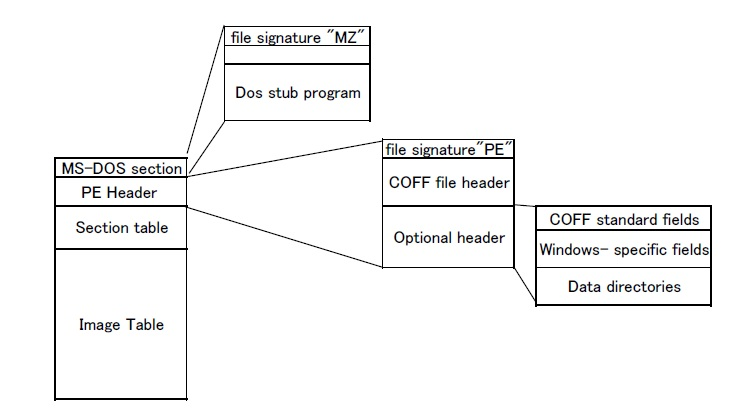
\includegraphics[width=1\textwidth]{graph/peheader1.jpg}
\caption{Layout a file in PE header format.}
\label{fig:peheader}
\end{figure}

The PE header starts with two characters "PE" as know as the PE header file signature.

The file header contains seven fields shown in Figure \ref{fig:fileheader}. The number of the members in section is determined by \emph{NumberOfSection} file in file header. 

\begin{figure}[h!]
\begin{center}
\begin{tabular}{ l | l | l }
Member & Offset & Size\\ \hline
Machine & 000000DC & Word\\ 
NumberOfSections & 000000DE & Word\\ 
TimeDateStamp & 000000E0 & Dword\\ 
PointerToSymbolTable & 000000E4 & Dword\\ 
NumberOfSymbols & 000000E8 & Dword\\ 
SizeOfOptionalHeader & 000000EC & Word\\ 
Characteristics & 000000EE & Word\\
\end{tabular}
\end{center}
\caption{Layout of a file header}
\label{fig:fileheader}
\end{figure}

The following of the file header is the Optional header which consists of three parts. The first part is the COFF standard fields which contains the sizes of various parts of code and the \emph{AddressOfEntryPoint} which indicates the location of the entry point of the application and, the location of the end of the Import Address Table(IAT).

In order to create a fast malware classification system, classification malware system based on PE header's meta-data.

\section{Decision tree\cite{wikipedia}}
Decision tree is a algorithm generally used in machine learning technique. Decision tree is to create a model that predicts the value of a target variable based on several input variables. An example is shown on the right. Each interior node corresponds to one of the input variables; there are edges to children for each of the possible values of that input variable. Each leaf represents a value of the target variable given the values of the input variables represented by the path from the root to the leaf.

In data mining, trees can be described also as the combination of mathematical and computational techniques to aid the description, categorization and generalization of a given set of data.
Data comes in records of the form
\(\textbf{x},Y\) = \(x_1, x_2, x_3, ..., x_k, Y\)
The dependent variable, Y, is the target variable is analysed to understand, classify or generalise. The vector x is composed of the input variables, x1, x2, x3, that are used for that task.
\section{Classification based on malware's meta-data using decision tree approach}
To make malware classification rapid and correct, decision tree algorithm is used in malware classification system.

As the previous section, Data comes in records of the form:
\(\textbf{x},Y\) = \(x_1, x_2, x_3, ..., x_k, Y\)
In malware classification system, Y is malware families name, \(x_1, x_2, x_3, ..., x_k, Y\) is meta-data. Malware name is provided by anti-virus engines that presented in chapter \ref{chap:2} cannot used in this system. The new malware families is required for detect meaningful characterization of malware. This classification system use famous malware families that reported in Information technology agency such as netsky, mydoom, autorun, mytob, and other famous malware families. Therefore, when new malware is classified into famous malware families, researcher detect some meaningful characterize of malware, and reduce time for malware analysis. 

